\documentclass[a4paper,11pt]{article}
\usepackage[authoryear]{natbib}
\usepackage{graphicx}

% define the title
\author{T. Kooij}
\title{Simulatie van fotondetectie in HiSPARC}
\begin{document}
% generates the title
\maketitle
% insert the table of contents
\tableofcontents

\section{Samenvatting}
Ja, het kan!

\section{Inleiding}
Geladen leptonen (elektronen en muonen) worden in HiSPARC stations efficient gedetecteerd met vinyltolueen scintilatorplaten. Doordat geladen deeltjes zeer veel interacties met materie hebben verliezen ze veel energie in de dectector. De detectie kans is 1 en de energieafgifte per deeltje is reproduceerbaar.

Detectie van fotonen is moeizaam. De werkzame doorsnedes van de interacties zijn klein, zodat de kans op interactie slechts enkele procentpunt is \citep*{Pennink:2010}. De energieafgifte per interactie kan echter groot zijn. Daarom is de energieafgifte per foton variabel.

In een pulsehoogtehistogram van een HiSPARC detector station zijn bijdragen van fotonen te identificeren \citep*{Pennink:2010}. In de simulatie van EAS op HiSPARC detectoren met behulp van CORSIKA en sapphire wordt geen rekening gehouden met de bijdragen van fotonen. Fotonen zijn wel aanwezig in de CORSIKA output, maar worden niet meegenomen in sapphire. Daarom is de interactie van fotonen met de HiSPARC detectoren onderzocht om de detectorreponse op fotonen in the bouwen in de sapphire simulaties.

\section{Theorie}
In de HiSPARC scintilator platen word fotonen (gamma's) gedetecteerd met een energie tussen 100 keV en 10 MeV \citep*{Steijger2010-gammas}. Er zijn drie mechanismen waarmee dergelijke gamma's energieverliezen in een scintilatorplaat: Het foto-elektrisch effect, compton verstrooiing en paarvorming. Door deze interacties wordt energie van de invallende fotonen ovegedragen aan elektronen in de detector. Deze elektronen worden dan gedetecteerd zoals invallende elektronen uit EAS.

De werkzame doorsnede voor het foto-elektrisch effect is alleen bij lage energie voldoende groot. Voor foton met energie rond 1 MeV is de werkzame doorsnede zo klein dat de interactie kans vrijwel nul is. Er zijn alleen FE interacties die elektronen met lage energie vrijmaken. De pulshoogte in de PMT is kleiner dan het ruisniveau. Citation-needed. Het foto-elektrisch effect kan buiten beschouwing gelaten worden.

Compton verstrooiing is de domineerende interactie. De elektronen die door deze interactie worden vrijegemaakt leveren pulshoogten tussen ruis-niveau en 1.x MIP. Compton verstrooiing moet worden gesimuleerd in de detector response voor fotonen.

Paar-vorming kan alleen optreden bij foton energie groter dan 1.022 MeV (de rustmassa van een elektron positron paar). De bijbehorende pulshoogtes zijn groot; In de orde van 1 MIP of meer. De werkzame doorsnede van paarvorming is klein, daarom is de interactiekans klein. De pulsen zijn in de detector ononderscheidbaar van pulsen die veroozaakt worden door invallende geladen leptonen. Hierdoor is de invloed van paar-vorming op het uiteindelijke pulseintegral histrogram minimaal. Paarvorming kan buiten beschouwng gelaten worden.


\section{Monte carlo simulatie van fotonen door een scintilatorplaat}

\subsection{Beschrijving van de montecarlo analyse}
Voor het analyseren van de response van HiSPARC detectoren op fotonen is een monte carlo simulatie programma geschreven door J. Steijger \citep*{Steijger2010-gammas}. De analyse wordt door de auteur \textit{mini montecarlo} genoemd.

De simulatie, geschreven in C, is gecompileerd met gcc-4.8.1 via cygwin64 op Windows 7. De uitvoer van de simulatie is of meerdere regels tekst per vrijgemaakt elektron. De opbouw van de tekstregels van de programmauitvoer is gedocumenteerd VERWIJS Github. De uitvoer wordt ingelezen een python-2.7 script waarmee de tabellen en figuren uit dit pamflet zijn gemaakt. De C en python broncode zijn beschikbaar via Github.

Aangenomen wordt dat de gammastraling loodrecht invalt op de detector en dat alle deeltje in dezelfde richting door de detector verplaatsen. De detector kan zo gemodelleerd worden als eendimensionaal met een lengte van 2,0 cm. De code simuleert een groot aantal fotonen waarvan de energie willekeurig getrokken wordt uit een 1/E verdeling tussen 100keV en 10MeV. Per foton wordt de werkzame doorsnede van de drie interacties bepaald en daaruit de vrije weglengte van het foton. De kleinste vrije wegelengte bepaalt het interactietype en een willekeurig getal bepaalt de interactieplaats. De aan de elektronen overgedragen energie wordt bepaald en daaruit wordt de aan de scintilatorplaat afgegeven energie berekend volgens de \textit{continuous slowing down approach} met dE/dx = 1.75 g/cm. Hierbij wordt zoals eerder genoemd aangenomen dat de elektronen ook loodrecht op scintilator plaat verder bewegen. Deze aanname is juist VERWIJZEN.

\subsection{Resultaten mini montecarlo}
De resultaten zijn allereerst uitgesplits per mechanisme, zie \ref{table:mmc-mechanisme}.
\begin{table}[ht]
\caption{Resultaten mini montecarlo}
\centering
\begin{tabular}{l c c c} % centered columns
\hline\hline
Omschrijving & aantal & percentage \\ [0.5ex] % header
\hline % inserts single horizontal line
Aantal primaire fotonen & 651075 & 100\% & - \\ % inserting body of the table
Fotonen met interactie & 100000 & 15.4\% & 100\% \\
waarvan foto-elektrischeffect & 293 & & 0.29\% \\
waarvan Compton verstrooing & 90596 & & 91\% \\
waarvan Paar vorming & 9111 & & 9.1\% \\ [1ex] % [1ex] adds vertical space
\hline %inserts single line
\end{tabular}
\label{table:mmc-mechanisme} % is used to refer this table in the text
\end{table}

\begin{figure}[t]
  \begin{center}
    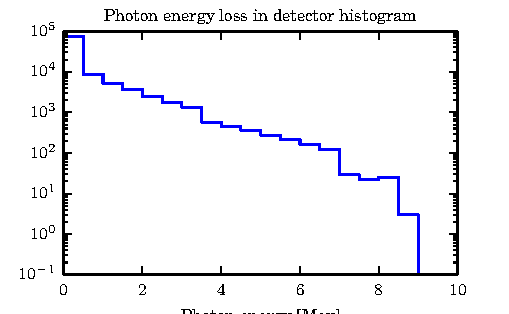
\includegraphics{figure1.pdf}
    \caption{\label{fig:Eloss-hist} Photon energy loss histogram.}
  \end{center}
\end{figure}



\subsection{analyse van FE-effect}
Uit de theorie wordt veronderstelt dat het FE-effect geen invloed heeft op de detectie van fotonen in HiSPARC, omdat PMT pulsen binnen het ruisniveau vallen.

Om deze aanname te toesen is het FE-effect uitgeschakeld in de montecarlo simulatie. De uitvoer van een run met en zonder FE-effect met dezelfde \textit{randomseed} is vergeleken. In de figuur (WELKE FIGUUR) is te zien dat het FE-effect BLABLABLA.

\subsection{analyse van Compton verstrooiing}
Hier moet bijvoorbeeld in dat alle energie van de elektronen wordt afgegeven in de detector.
\subsection{analyse van Paarvorming}

\section{Compton verstrooiing}
Uitleg compton verstrooing

Deze paragraaf vullen naar behoefte vanuit tekst hieronder
\subsection{Detectiekans}
Werkzamedoorsnede
\subsection{Afgegeven energie aan het electron}

\section{Parametrisatie}
\subsection{Detectiekans}
\subsection{Afgegeven energie}

\section{Sapphire algorithme}
Flowchart?


\bibliography{mybib}{}
\bibliographystyle{plain}


\end{document}
